\chapter{Int\'egration des \'equations du mouvement}

\section{Mouvement lin\'eaire}

L'\'equation (\ref{EQ:5_5}) appliqu\'ee \`a un point mat\'eriel donne en coordonn\'ees g\'en\'eralis\'ees :
\be
	L = \frac{1}{2}a(q)\dot{q}^{2} - U(q) \label{EQ:11_1}
\ee
qui s'\'ecrit en coordonn\'ees cart\'esiennes :
\be
	L = \frac{1}{2}m\dot{x}^{2} - U(x) \label{EQ:11_2}
\ee
En \'ecrivant l'\'energie totale :
\bea
	E = T + U & = & \frac{1}{2}m\dot{x}^{2} + U(x) \nonumber \\
	\dot{x}^{2} & = & \frac{2}{m}(E-U(x)) \nonumber \\
	\dfrac{\mathrm{d}x}{\mathrm{dt}} & = & \sqrt{\frac{2}{m}(E-U(x))} \nonumber \\
	t & = & \sqrt{\frac{m}{2}}\bigintsss{\dfrac{\mathrm{d}x}{\sqrt{E-U(x)}}} + cste \label{EQ:11_3}
\eea
o\`u $E$ et $cste$ sont des constantes du mouvement, la premi\`ere par la loi de conservation de l'\'energie et la seconde par int\'egration.

Lors d'un mouvement, l'\'energie totale est toujours sup\'erieure \`a l'\'energie potentielle car l'\'energie cint\'etique ne peut \^etre n\'egative. Aussi le mouvement ne peut \^etre possible que si $U(x)<E$.

\begin{figure}[htb!]
	\begin{center}
		\begin{picture}(200,150)(0,0)
			%axis
			\linethickness{0.05mm}
			\put(0,0){\line(1,0){200}}\put(202,-2){$x$}
			\put(0,0){\line(0,1){140}}\put(-2,142){$U$}
			%curve
			\linethickness{0.5mm}
			\qbezier(-5,130),(15,130),(25,110)
			\qbezier(25,110),(35,90),(55,90)
			\qbezier(55,90),(80,90),(90,100)
			\qbezier(90,100),(100,110),(125,110)
			\qbezier(125,110),(150,110),(190,20)
			%limit
			\linethickness{0.05mm}
			\multiput(-5,100)(10,0){20}{\line(1,0){8}}\put(195,98){$U=E$}
			\multiput(32,0)(0,5){20}{\line(0,1){3}}\put(34,102){$A$}\put(28,-7){$x_{1}$}
			\multiput(90,0)(0,5){20}{\line(0,1){3}}\put(82,102){$B$}\put(86,-7){$x_{2}$}
			\put(142,102){$C$}
		\end{picture}
		\caption{Exemple d'une fonction d\'efinissant l'\'energie potentielle}\label{FIG:3_1}
	\end{center}
\end{figure}

Sur la figure (\ref{FIG:3_1}), la condition $U(x)<E$ implique que le mouvement n'est possible que sur les intervalles tels que $x\in\left[A\,;B\right]$ et $x\in\left[C\,;+\infty\right[$. Dans le premier cas, le mouvement est dit fini et oscillatoire. Dans le second cas, le mouvement est dit inifini. Les points tels que :
\be
	U(x) = E \label{EQ:11_4}
\ee
sont les \emph{points d'arr\^et}. En effet, dans ce cas, l'\'energie cin\'etique du point mat\'eriel est nulle car sa vitesse aussi de facto.

Dans la relation (\ref{EQ:5_1}), nous avons vu que le temps n'est pas qu'uniforme, il est aussi isotrope. Ainsi la transformation $\mathrm{t}\mapsto -\mathrm{t}$ laisse inchang\'ee la fonction de Lagrange et les \'equations du mouvement. Ainsi $\Delta\mathrm{t}(x_{1}\rightarrow x_{2}) = \Delta\mathrm{t}(x_{2}\rightarrow x_{1})$ et la période d'oscillation $\mathrm{T}(E)=\Delta\mathrm{t}(x_{1}\rightarrow x_{2}\rightarrow x_{1})$ vaut $2\Delta\mathrm{t}(x_{1}\rightarrow x_{2})$. L'\'equation (\ref{EQ:11_3}) s'\'ecrit alors :
\bea
	\mathrm{T}(E) & = & 2\sqrt{\frac{m}{2}}\bigintsss_{x_{1}(E)}^{x_{2}(E)}{\dfrac{\mathrm{d}x}{\sqrt{E-U(x)}}} \nonumber \\
	\mathrm{T}(E) & = & \sqrt{2m}\bigintsss_{x_{1}(E)}^{x_{2}(E)}{\dfrac{\mathrm{d}x}{\sqrt{E-U(x)}}}\label{EQ:11_5}
\eea
qui d\'etermine la p\'eriode d'oscillation de la particule mat\'erielle en fonction de son \'energie totale.

\section{D\'efinition de l'\'energie potentielle en fonction de la p\'eriode des oscillations}

\begin{figure}[htb!]
	\begin{center}
		\begin{picture}(200,150)(0,0)
			%axis
			\linethickness{0.05mm}
			\put(0,0){\line(1,0){200}}\put(202,-2){$x$}
			\put(100,0){\line(0,1){140}}\put(98,142){$U$}
			%curve
			\linethickness{0.5mm}
			\qbezier(35,120),(40,0),(100,0)
			\qbezier(100,0),(175,0),(180,120)
			\put(47,50){$x_{1}(U)$}
			\put(132,50){$x_{2}(U)$}
			%limit
			\linethickness{0.05mm}
			\multiput(-5,80)(10,0){20}{\line(1,0){8}}\put(195,78){$U=E$}
			\multiput(40,0)(0,5){16}{\line(0,1){3}}\put(35,-7){$x_{1}$}
			\multiput(175,0)(0,5){16}{\line(0,1){3}}\put(170,-7){$x_{2}$}
		\end{picture}
		\caption{Fonction d\'efinissant l'\'energie potentielle ayant qu'un unique minimum}\label{FIG:3_2}
	\end{center}
\end{figure}

L'objectif de ce paragraphe est de trouver la fonction d\'efinissant l'\'energie potentielle d'un champ $U$ connaissant la p\'eriode d'oscillations $\mathrm{T}(E)$ du mouvement animant une particule. Pour cela, nous supposons que la fonction recherch\'ee $U$ n'a qu'un unique minimum dans la r\'egion du mouvement et que, comme sur la figure (\ref{FIG:3_2}), $U(0) = 0$.

Transformons l'int\'egrale (\ref{EQ:11_5}) avec $x$ fonction de $U$ telle que pour une valeur de l'\'energie potentielle $U$ il existe deux valeurs de $x$ diff\'erentes. Elle devient alors la somme de deux int\'egrales sur deux r\'egions diff\'erentes :
\bea
	\mathrm{T}(E) & = & \sqrt{2m}\bigintsss_{x_{1}(E)}^{x_{2}(E)}\dfrac{\mathrm{d}x}{\sqrt{E - U(x)}} \nonumber \\
	& = & -\sqrt{2m}\bigintsss_{0}^{E}\dfrac{\mathrm{d}x_{1}}{\mathrm{d}U}\dfrac{\mathrm{d}U}{\sqrt{E - U}} + \sqrt{2m}\bigintsss_{0}^{E}\dfrac{\mathrm{d}x_{2}}{\mathrm{d}U}\dfrac{\mathrm{d}U}{\sqrt{E - U}} \nonumber \\
	& = & \sqrt{2m}\bigintsss_{0}^{E}\left[\dfrac{\mathrm{d}x_{2}}{\mathrm{d}U} - \dfrac{\mathrm{d}x_{1}}{\mathrm{d}U}\right]\dfrac{\mathrm{d}U}{\sqrt{E - U}}
\eea
Elle peut \^etre \'etendue \`a :
\bea
	\bigintsss_{0}^{\alpha}\dfrac{\mathrm{T}(E)\mathrm{d}E}{\sqrt{\alpha - E}} & = & \sqrt{2m}\bigintsss_{0}^{\alpha}\bigintsss_{0}^{E}\left[\dfrac{\mathrm{d}x_{2}}{\mathrm{d}U} - \dfrac{\mathrm{d}x_{1}}{\mathrm{d}U}\right]\dfrac{\mathrm{d}U\mathrm{d}E}{\sqrt{(\alpha - E)(E - U)}} \nonumber \\
	& =& \sqrt{2m}\bigintsss_{0}^{\alpha}\left[\dfrac{\mathrm{d}x_{2}}{\mathrm{d}U} - \dfrac{\mathrm{d}x_{1}}{\mathrm{d}U}\right]\mathrm{d}U\bigintsss_{U}^{\alpha}\dfrac{\mathrm{d}E}{\sqrt{(\alpha - E)(E - U)}}
\eea
La seconde implication dans sa deuxi\`eme int\'egrale est en $\int_{U}^{\alpha}$ car en dehors de cet intervalle, $\int_{0}^{U}$ et $\int_{\alpha}^{E}$ sont ind\'efinie car $(E-U)$ et $(\alpha-E)$ sont respectivement n\'egatives.

Faisons d\'esormais le calcul de la seconde int\'egrale, soit :
\be
	\bigintsss_{U}^{\alpha}\dfrac{\mathrm{d}E}{\sqrt{(\alpha - E)(E - U)}}
\ee
en posant :
\be
	y = \dfrac{2E - U - \alpha}{\alpha - U}
\ee
qui donne :
\be
	\begin{cases}
		E = \dfrac{(\alpha - U)y + U + \alpha}{2} \\
		\mathrm{d}y = \dfrac{2\mathrm{d}E}{\alpha - U} \Leftrightarrow \mathrm{d}E = \dfrac{\alpha - U}{2}\mathrm{d}y
	\end{cases}
\ee
et :
\be
	\begin{cases}
		E = U \Rightarrow y = \dfrac{U - \alpha}{\alpha - U} = -1 \\
		E = \alpha \Rightarrow y = \dfrac{-U + \alpha}{\alpha - U} = 1
	\end{cases}
\ee
Ainsi :
\bea
	\bigintsss_{U}^{\alpha}\dfrac{\mathrm{d}E}{\sqrt{(\alpha - E)(E - U)}} & = & \bigintsss_{-1}^{1}\dfrac{(\alpha - U)\mathrm{d}y}{2\sqrt{\frac{(2\alpha - (\alpha - U)y + U + \alpha)}{2}\frac{((\alpha - U)y + U + \alpha - 2U)}{2}}} \nonumber \\
	& = & \bigintsss_{-1}^{1}\dfrac{(\alpha - U)\mathrm{d}y}{2\sqrt{\frac{(\alpha - U - (\alpha - U)y)}{2}\frac{(\alpha - U + (\alpha - U)y)}{2}}} \nonumber \\
	& = & \bigintsss_{-1}^{1}\dfrac{(\alpha - U)\mathrm{d}y}{2\frac{\alpha - U}{2}\sqrt{(1 - y)(1 + y)}} = \bigintsss_{-1}^{1}\dfrac{\mathrm{d}y}{\sqrt{1 - y^{2}}}
\eea
En posant $u = y^{2}$ soit $y = u^{1/2}$ et $\mathrm{d}u = 2y\mathrm{d}y = 2u^{1/2}\mathrm{d}y \Leftrightarrow \mathrm{d}y = \frac{1}{2}u^{-1/2}\mathrm{d}u$, l'int\'egrale pr\'ec\'edente s'\'ecrit :
\bea
	\bigintsss_{U}^{\alpha}\dfrac{\mathrm{d}E}{\sqrt{(\alpha - E)(E - U)}} & = & \bigintsss_{-1}^{1}\dfrac{\mathrm{d}y}{\sqrt{1 - y^{2}}} = 2 \bigintsss_{0}^{1}\dfrac{1}{2}\dfrac{u^{-1/2}\mathrm{d}u}{(1-u)^{1/2}} \nonumber \\
	& = & \int_{0}^{1}u^{-1/2}(1-u)^{-1/2}\mathrm{d}u \nonumber \\
	& = & \mathrm{B}\left(\dfrac{1}{2},\dfrac{1}{2}\right) = \dfrac{\Gamma(\dfrac{1}{2})\Gamma(\dfrac{1}{2})}{\Gamma(1)} = \pi
\eea
De fait :
\bea
	\bigintsss_{0}^{\alpha}\dfrac{\mathrm{T}(E)\mathrm{d}E}{\sqrt{\alpha - E}} & = & \sqrt{2m}\pi\bigintsss_{0}^{\alpha}\left[\dfrac{\mathrm{d}x_{2}}{\mathrm{d}U} - \dfrac{\mathrm{d}x_{1}}{\mathrm{d}U}\right]\mathrm{d}U \nonumber \\
	& = & \sqrt{2m}\pi\left[x_{2}(\alpha) - x_{2}(0) - x_{1}(\alpha) + x_{1}(0)\right]
\eea
Or par hypoth\`ese, $x_{2}(0) = x_{1}(0) = 0$, donc :
\be
	\bigintsss_{0}^{\alpha}\dfrac{\mathrm{T}(E)\mathrm{d}E}{\sqrt{\alpha - E}} = \sqrt{2m}\pi\left[x_{2}(\alpha) - x_{1}(\alpha)\right]
\ee
Dans le cas o\`u nous posons $\alpha = U$, nous pouvons en d\'eduire :
\be
	x_{2}(U) - x_{1}(U) = \dfrac{1}{\sqrt{2m}\pi}\bigintsss_{0}^{U}\dfrac{\mathrm{T}(E)\mathrm{d}E}{\sqrt{U - E}} \label{EQ:12_1}
\ee
De plus, si le champ d'\'energie potentielle est paire tel que $U(x) = U(-x)$ ou encore $x_{1}(U) = -x_{2}(U) = x(U)$, alors l'\'equation (\ref{EQ:12_1}) devient, puisque $x_{2}(U) - x_{1}(U) = 2x(U)$ :
\be
	x(U) = \dfrac{1}{2\pi\sqrt{2m}}\bigintsss_{0}^{U}\dfrac{\mathrm{T}(E)\mathrm{d}E}{\sqrt{U - E}} \label{EQ:12_2}
\ee

\section{Masse r\'eduite}

L'important probl\`eme du mouvement s'un syst\`eme ferm\'e \`a deux particules r\'eagissant l'une sur l'autre, ou encore \emph{probl\`eme des deux corps}, admet une solution g\'en\'erale compl\`ete. Pour le r\'esoudre, nous allons le simplifier en d\'ecomposant le mouvement du syst\`eme en celui du centre d'inertie et des deux points mat\'eriels par rapport \`a ce dernier. L'\'energie potentielle d'int\'eraction ne d\'epend que de la distance entre les deux particules, aussi la fonction de Lagrange s'\'ecrit :
\be
	L = \dfrac{m_{1}\dot{r}_{1}^{2}}{2} + \dfrac{m_{2}\dot{r}_{2}^{2}}{2} - U(\lvert \vec{r}_{1} - \vec{r}_{2} \rvert) \label{EQ:13_1}
\ee
D\'efinissons $\vec{r} = \vec{r}_{1} - \vec{r}_{2}$ et pla\c{c}ons l'origine des coordonn\'ees au centre d'inertie. Alors l'\'equation (\ref{EQ:8_3}) donne $\vec{R} = \vec{0}$ ou encore : $\sum m_{a}\vec{r}_{a} = \vec{0}$, soit :
\be
	m_{1}\vec{r}_{1} + m_{2}\vec{r}_{2} = \vec{0}
\ee
Nous pouvons en conclure que :
\be
	\vec{r} = \begin{cases}
		\vec{r}_{1} + \dfrac{m_{1}}{m_{2}}\vec{r}_{1} = \dfrac{m_{1} + m_{2}}{m_{2}}\vec{r}_{1} \\
		- \dfrac{m_{2}}{m_{1}}\vec{r}_{2} - \vec{r}_{2} = -\dfrac{m_{1} + m_{2}}{m_{1}}\vec{r}_{2}
	\end{cases}
\ee
soit :
\be
	\begin{cases}
		\vec{r}_{1} = \dfrac{m_{2}}{m_{1} + m_{2}}\vec{r} \\
		\vec{r}_{2} = \dfrac{-m_{1}}{m_{1} + m_{2}}\vec{r}
	\end{cases}\label{EQ:13_2}
\ee
Puisque :
\be
	\begin{cases}
		\vec{\dot{r}}_{1} = \dfrac{m_{2}}{m_{1} + m_{2}}\vec{\dot{r}} \\
		\vec{\dot{r}}_{2} = \dfrac{-m_{1}}{m_{1} + m_{2}}\vec{\dot{r}}
	\end{cases}
\ee
la fonction de Lagrange se d\'eveloppe ainsi :
\bea
	L & = & \dfrac{m_{1}}{2}\left(\dfrac{m_{2}}{m_{1} + m_{2}}\right)^{2}\vec{\dot{r}}^{\,2} + \dfrac{m_{2}}{2}\left(\dfrac{-m_{1}}{m_{1} + m_{2}}\right)^{2}\vec{\dot{r}}^{\,2} - U(\vec{r}) \nonumber \\
	& = & \dfrac{m_{1}m_{2}^{2} + m_{1}^{2}m_{2}}{2(m_{1} + m_{2})^{2}}\vec{\dot{r}}^{\,2} - U(\vec{r}) = \dfrac{m_{1}m_{2}(m_{2} + m_{1})}{2(m_{1} + m_{2})^{2}}\vec{\dot{r}}^{\,2} - U(\vec{r})
\eea
et on peut conclure en posant \emph{la masse r\'eduite} :
\be
	m = \dfrac{m_{1}m_{2}}{(m_{1} + m_{2})} \label{EQ:13_4}
\ee
\`a :
\be
	L = \dfrac{m}{2}\vec{\dot{r}}^{\,2} - U(\vec{r}) \label{EQ:13_3}
\ee
qui est la fonction de Lagrange d'un point mat\'eriel de masse $m$ se d\'epla\c{c}ant dans le champ ext\'erieur $U(\vec{r})$ qui est sym\'etrique par rapport au point immobile des coordonn\'ees, soit le centre d'inertie. Ainsi le calcul de $\vec{r} = \vec{r}(\mathrm{t})$ permet gr\^ace aux \'equations (\ref{EQ:13_2}) d'en d\'eduire les trajectoires $\vec{r}_{1}(\mathrm{t})$ et $\vec{r}_{2}(\mathrm{t})$ des particules de masse respective $m_{1}$ et $m_{2}$.

\section{Mouvement dans un champ central}

Le fait de ramener le probl\`eme \`a deux corps \`a celui d'un seul nous conduit \`a devoir d\'eterminer le mouvement d'une particule dans un champ ext\'erieur o\`u son \'energie potentielle ne d\'epend que de la distance $r$ \`a un point immobile. Ce champ est appel\'e \emph{champ central}. De la relation (\ref{EQ:5_4}), la force est donn\'ee par :
\be
	\vec{F} = -\dfrac{\partial U(r)}{\partial\vec{r}} = -\dfrac{\mathrm{d}U(r)}{\mathrm{d}r}\dfrac{\vec{r}}{r}
\ee
et agissant sur la particule, elle ne d\'epend aussi que de $r$.

Par d\'efinition, \'equation (\ref{EQ:9_3}), le moment cin\'etique est :
\be
	\vec{M} = \vec{r}\wedge\vec{p}
\ee
et dans un champ central, il se conserve dans un r\'ef\'erentiel dont un axe passe par le centre et ce dernier est le centre du r\'ef\'erentiel. Dans ce cas de conservation et parce que $\vec{M}\perp\vec{p}$ alors le mouvement de la particule reste toujours dans le m\^eme plan perpendiculaire au moment cin\'etique. Ainsi, en coordonn\'ees polaires (cylindriques), nous avons de facto $\dot{z} = 0$ et la fonction de Lagrange est, voir l'\'equation (\ref{EQ:4_5}) :
\be
	L = \dfrac{m}{2}(\dot{r}^{2} + r^{2}\dot{\varphi}^{2}) - U(r) \label{EQ:14_1}
\ee
La coordonn\'ee $\varphi$ est dite \emph{cyclique} car elle n'appara\^it pas explicitement dans la d\'efinition de la fonction de Lagrange, alors que $r$ et $\dot{\varphi}$ en sont des coordonn\'ees \emph{principales}. Pour la coordonn\'ee $\varphi$, les \'equations de Lagrange (\ref{EQ:2_6}) sont :
\be
	\dfrac{\mathrm{d}}{\mathrm{dt}}\left(\dfrac{\partial L}{\partial\dot{q}_{i}}\right) = \dfrac{\partial L}{\partial q_{i}} = 0
\ee
Ainsi, l'impulsion g\'en\'eralis\'ee, \'equation (\ref{EQ:7_5}) :
\be
	p_{i} = \dfrac{\partial L}{\partial\dot{q}_{i}}
\ee
est constante dans le temps, i.e. $p_{i}$ est une int\'egrale premi\`ere, soit une int\'egrale du mouvement qui conserve sa valeur pendant le mouvement. L'\'equation (\ref{EQ:14_1}) permet d'\'ecrire\footnote{Il s'agit bien de $p_{\varphi}$ et non pas de $\dot{p}_{\varphi}$ commme inscrit dans le livre.} :
\be
	\dfrac{\partial L}{\partial\dot{q}_{i}} = mr^{2}\dot{\varphi} = p_{\varphi}
\ee
et la valeur de $p_{\varphi}$ se conserve dans le temps. En appliquant l'\'equation (\ref{EQ:9_7}) car nous avons choisi le r\'ef\'erentiel tel que la particule tourne dans un plan perpendiculaire \`a un axe passant par le centre du champ :
\bea
	M_{z} & = & \dfrac{\partial L}{\partial\dot{\varphi}_{i}} \nonumber \\
	\Leftrightarrow M & = & mr^{2}\dot{\varphi} \label{EQ:14_2}
\eea
Car les valeurs de $M$ et de $M_{z}$ se confondent par d\'efinition du choix fait pr\'ec\'edemment. La valeur de $M$ est donc conserv\'ee \'egalement. $\dot{\varphi}$ ne changeant pas de signe au cours du mouvement\footnote{En effet, $M$ est une valeur constante, commme $m$ alors que $r^{2}$ est toujours positive.}, $\varphi$ \'evolue de mani\`ere monotone.

\begin{figure}[htb!]
	\begin{center}
		\begin{picture}(200,150)(0,0)
			%curve
			\linethickness{0.5mm}
			\qbezier(120,150),(150,125),(170,75)
			\qbezier(170,75),(180,50),(190,5)
			%vectors
			\linethickness{0.05mm}
			\put(-8,47){$0$}
			\put(0,50){\vector(1,0){178}}
			\put(75,80){$\vec{r}$}
			\put(0,50){\vector(8,2){163}}
			%tangent
			\multiput(162,50)(0,5){8}{\line(0,1){3}}
			\put(135,65){$r\mathrm{d}\varphi$}
			%angle
			\qbezier(25,50),(25,55),(20,55)
			\put(27,52){$\mathrm{d}\varphi$}
		\end{picture}
		\caption{Aire balay\'ee}\label{FIG:3_7}
	\end{center}
\end{figure}

R\'efl\'echissons d\'esormais à l'interpr\'etation g\'eom\'etrique de la loi pr\'ec\'edente (\ref{EQ:14_2}) en remarquant que l'expression $\frac{1}{2}\vec{r}\cdot\vec{r}\mathrm{d}\varphi$ repr\'sente la surface form\'ee par les deux rayons vecteurs infiniment voisins et l'arc de la trajectoire de la figure (\ref{FIG:3_9}). En d\'esignant par $\mathrm{d}f$ cet \'el\'ement de surface, le moment cin\'etique de la particule devient :
\be
	M = 2m\dot{f} \label{EQ:14_3}
\ee
car en s'aidant de la relation (\ref{EQ:14_2}) :
\bea
	\mathrm{d}f & = & \dfrac{1}{2}\vec{r}\cdot\vec{r}\mathrm{d}\varphi = \dfrac{1}{2}r^{2}\mathrm{d}\varphi \nonumber \\
	\dot{f} = \dfrac{\mathrm{d}f}{\mathrm{dt}} & = & \dfrac{1}{2}r^{2}\dot{\varphi} \nonumber
\eea
La grandeur $\dot{f}$ est alors appel\'ee \emph{vitesse a\'erolaire}. Et comme le moment cin\'etique $M$ est constant pendant le mouvement alors la vitesse a\'erolaire est constante \'egalement, il s'agit de la \emph{seconde loi de Kepler}, \`a savoir que pendant des intervalles de temps \'egaux, le rayon vecteur d'un point mobile balaye des aires \'egales. Cette seconde loi est aussi appel\'ee \emph{int\'egrale des aires} qui est la loi de conservation du moment cin\'etique d'une particule en mouvement dans un champ central.

Pour obtenir la solution compl\`ete du mouvement d'une particule dans un champ central, utilisons les lois de conservation de l'\'energie (\'equation (\ref{EQ:6_1}) et du moment cin\'etique (\'equation (\ref{EQ:9_3}). D'apr\`es la relation (\ref{EQ:14_2}), $\dot{\varphi} = \frac{M}{mr^{2}}$, donc l'\'energie peut s'\'ecrire comme :
\be
	E = T + U = \dfrac{m}{2}(\dot{r}^{2} + r^{2}\dot{\varphi}^{2}) + U(r) = \dfrac{m}{2}\dot{r}^{2} + \dfrac{M^{2}}{2mr^{2}} + U(r) \label{EQ:14_4}
\ee
qui implique directement :
\be
	\dot{r} = \dfrac{\mathrm{d}r}{\mathrm{dt}} = \pm\sqrt{\frac{2}{m}(E - U(r)) - \frac{M^{2}}{m^{2}r^{2}}} \label{EQ:14_5}
\ee
En renversant, nous obtenons :
\be
	\mathrm{dt} = \dfrac{\mathrm{d}r}{\sqrt{\frac{2}{m}(E - U(r)) - \frac{M^{2}}{m^{2}r^{2}}}}
\ee
qui permet d'obtenir par intégration :
\be
	t = \bigintsss{\dfrac{\mathrm{d}r}{\sqrt{\frac{2}{m}(E - U(r)) - \frac{M^{2}}{m^{2}r^{2}}}}} + cste \label{EQ:14_6}
\ee
En reprenant l'\'equation (\ref{EQ:14_2}) sous la forme :
\bea
	M & = & mr^{2}\dot{\varphi} \nonumber \\
	\mathrm{d}\varphi & = & \dfrac{M}{mr^{2}}\mathrm{dt}
\eea
et en l'injection dans la relation (\ref{EQ:14_5}), nous avons :
\bea
	\dfrac{\mathrm{d}r}{\mathrm{dt}} = \dfrac{M\mathrm{d}r}{mr^{2}\mathrm{d}\varphi} & = & \sqrt{\frac{2}{m}(E - U(r)) - \frac{M^{2}}{m^{2}r^{2}}} \nonumber \\
	\Leftrightarrow \mathrm{d}\varphi & = & \dfrac{M\mathrm{d}r}{mr^{2}\sqrt{\frac{2}{m}(E - U(r)) - \frac{M^{2}}{m^{2}r^{2}}}} \nonumber \\
	& = & \dfrac{\frac{M}{r^{2}}\mathrm{d}r}{\sqrt{2m(E - U(r)) - \frac{M^{2}}{r^{2}}}} \nonumber \\
	\Leftrightarrow \varphi & = & \bigintsss{\dfrac{\frac{M}{r^{2}}\mathrm{d}r}{\sqrt{2m(E - U(r)) - \frac{M^{2}}{r^{2}}}}} + cste \label{EQ:14_7}
\eea

Les formules (\ref{EQ:14_6}) et (\ref{EQ:14_7}) forment la solution g\'en\'erale. La premi\`ere donne implicitement la distance au centre $r$ en fonction du temps alors que la seconde \'etablit la relation entre $r$ et $\varphi$, soit l'\'equation du mouvement.

\begin{figure}[htb!]
	\begin{center}
		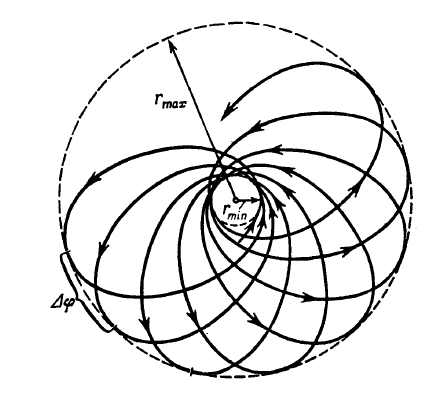
\includegraphics[width=10cm]{chapter_03_paragraph_14_fig_09}
		\caption{Trajectoire dans un champ central attracteur}\label{FIG:3_9}
	\end{center}
\end{figure}

L'\'equation (\ref{EQ:14_4}) :
\be
	E = T + U = \dfrac{m}{2}\dot{r}^{2} + \dfrac{M^{2}}{2mr^{2}} + U(r)
\ee
peut se r\'e\'ecrire en identifiant $\frac{m}{2}\dot{r}^{2}$ comme l'\'energie cin\'etique radiale de la particule comme :
\be
	E = \dfrac{m}{2}\dot{r}^{2} + U_{\mathrm{eff}}(r)
\ee
avec :
\be
	U_{\mathrm{eff}}(r) = \dfrac{M^{2}}{2mr^{2}} + U(r) \label{EQ:14_8}
\ee
se d\'efinissant comme une \'energie potentielle efficace o\`u le terme $\frac{M^{2}}{2mr^{2}}$ est l'\emph{\'energie centrifuge}. Ainsi, la partie radiale du mouvement de la particule peut \^etre consid\'er\'ee comme un mouvement lin\'eaire dans un champ dot\'e d'une \'energie potentielle efficace.

Les valeurs de la distance telle que l'\'energie cin\'etique radiale s'annule ou encore $E = U_{\mathrm{eff}}(r)$ d\'elimitent le domaine du mouvement de la particule car cela n\'ecessite de facto $\dot{r} = 0$. Cela d\'efinit les \emph{points de rebroussement} o\`u la particule peut encore avoir une vitesse angulaire $\dot{\varphi}\neq 0$. La fonction $r(\mathrm{t})$ devient ensuite croissante ou d\'ecroissante. Il existe alors deux possibilit\'es :
\begin{itemize}
	\item $r \gg r_{min}$ alors le mouvement est infini
	\item $r_{min} \leqslant r \leqslant r_{max}$ alors la trajectoire est contenue dans l'anneau d\'efini par les cercles de rayon $r_{min}$ et $r_{max}$
\end{itemize}
Dans le second cas, la variation angulaire $\Delta\varphi$ de la trajectoire de la particule pendant qu'elle fait le trajet $r_{max} \rightarrow r_{min} \rightarrow r_{max}$\footnote{Ou l'\'equivalent sym\'etrique $r_{min} \rightarrow r_{max} \rightarrow r_{min}$.} vaut d'apr\`es l'\'equation (\ref{EQ:14_7}) :
\be
	\Delta\varphi = 2\bigintsss_{r_{min}}^{r_{max}}{\dfrac{\frac{M}{r^{2}}\mathrm{d}r}{\sqrt{2m(E - U(r)) - \frac{M^{2}}{r^{2}}}}} \label{EQ:14_10}
\ee
La trajectoire de la particule est finie, i.e. elle se referme, si et seulement si $\Delta\varphi = \frac{m}{n}\times 2\pi$ avec ${m;n}\in\mathbb{N}$. Ainsi, quand le rayon vecteur parcourt $n$ p\'eriodes, il fait \'egalement $m$ tours complets et la trajectoire se referme. Toutefois, cela reste un cas particulier. En g\'en\'eral $U(r)$ ne permet par d'obtenir $\Delta\varphi$ comme une fraction rationnelle de $2\pi$ et la trajectoire ne se referme pas et finit par remplir tout l'espace de l'anneau compris entre $r_{min}$ et $r_{max}$. Finalement, la trajectoire est ferm\'ee pour les \'energies potentielles en $\frac{1}{r}$, voir le paragraphe \ref{PAR:15} et en $r^{2}$, voir l'exercice \ref{PAR:23_EX3}.

Aux points de rebroussement d\'efinis tels que $\dot{r} = 0$, il y a un changement de signe de la vitesse radiale et donc de la direction radiale prise par la particule. Que ce soit en $r_{min}$ ou $r_{max}$, la quantit\'e $\dfrac{\dot{r}(\mathrm{t} - \delta\mathrm{t})}{\dot{r}(\mathrm{t} + \delta\mathrm{t})}$ est n\'egative. La trajectoire est ainsi sym\'etrique par rapport \`a la direction indiqu\'ee.

Pour le mouvement d'une particule ayant une moment cin\'etique non nulle, la position $r=0$ est inatteignable car :
\be
	\lim_{r\rightarrow 0}\dfrac{M^{2}}{2mr^{2}} \rightarrow +\infty
\ee

L'\'equation (\ref{EQ:14_4}) implique de facto\footnote{Dans l'expression finale de cette s\'equence, le livre affiche le signe $<$ au lieu de $>$.} :
\bea
	E - U(r) - \dfrac{M^{2}}{2mr^{2}} & = & \dfrac{m\dot{r}^{2}}{2} > 0 \nonumber \\
	r^{2}E - r^{2}U(r) & > & \dfrac{M^{2}}{2m} \nonumber \\
	r^{2}E & > & r^{2}U(r) + \dfrac{M^{2}}{2m}
\eea

Par conservation de l'\'energie, nous avons si $\lim_{r\rightarrow 0} r^{2}E = 0$, aussi $r$ ne peut tendre vers 0 que si :
\bea
	0 & > & \lim_{r\rightarrow 0}(r^{2}U(r)) + \dfrac{M^{2}}{2mr^{2}} \nonumber \\
	\lim_{r\rightarrow 0}(r^{2}U(r)) & < & -\dfrac{M^{2}}{2mr^{2}} \label{EQ:14_11}
\eea
Et cette derni\`ere in\'egalit\'e n'est vraie que dans deux situations et implique que $r$ peut ainsi tendre vers le centre du champ d'\'energie potentielle :
\begin{itemize}
	\item $U(r)=\dfrac{-\alpha}{r^{2}}$ avec $\alpha > \dfrac{M^{2}}{2mr^{2}}$
	\item $U(r)=\dfrac{-\alpha}{r^{n}}$ avec $n > 2$ car $\lim_{r\rightarrow 0}(r^{2}U(r)) = \lim_{r\rightarrow 0}\left(\dfrac{-\alpha}{r^{n-2}}\right) = -\infty < -\dfrac{M^{2}}{2mr^{2}}$
\end{itemize}

\section{Le probl\`eme de Kepler}\label{PAR:15}

\subsection{G\'en\'eralit\'es}

L'\'etude du champ central inversement proportionnel \`a $r$ est tr\`es important\footnote{Cela correspond \`a une force inversement proportionnel au carr\'e de la distance, voir l'\'equation (\ref{EQ:7_4}) donnant $\vec{F} = \dfrac{\partial L}{\partial U}$} car il s'agit du champ gravitationnel, attractif, et du champ \'electrostatique de Coulomb, attractif ou r\'epulsif. Ainsi, d\'efinissons un champ d'attraction tel que :
\be
	U(r) = -\dfrac{\alpha}{r} \label{EQ:15_1}
\ee
avec la constante $\alpha > 0$. Selon la relation (\ref{EQ:14_8}), l'\'energie potentielle efficace s'\'ecrit alors :
\be
	U_{eff}(r) = -\dfrac{\alpha}{r} + \dfrac{M^{2}}{2mr^{2}} \label{EQ:15_2}
\ee
qui est repr\'esent\'ee sur la figure (\ref{FIG:3_10}).

\begin{figure}[htb!]
	\begin{center}
		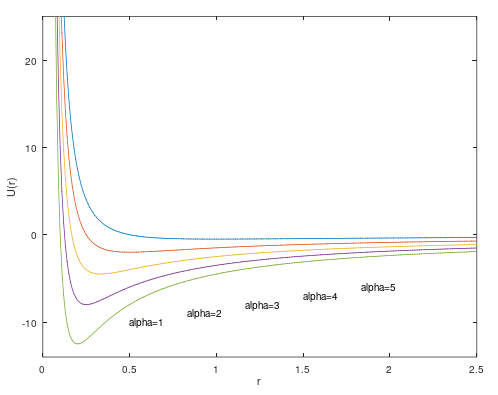
\includegraphics[width=10cm]{chapter_03_paragraph_15_fig_10}
		\caption{\'Energie potentielle attractrice pour $\alpha\in \{1;2;3;4;5\}$ et $M^{2}/m = 1$}\label{FIG:3_10}
	\end{center}
\end{figure}
Le minimum de la fonction pr\'ec\'edente s'obtient avec :
\bea
	\dfrac{\mathrm{d}U_{eff}(r)}{\mathrm{d}r} & = & 0 \Leftrightarrow \dfrac{\alpha}{r^{2}} - \dfrac{2M^{2}}{2mr^{3}} = 0 \nonumber \\
	\Leftrightarrow \dfrac{\alpha}{r^{2}} & = & \dfrac{M^{2}}{mr^{3}} \Leftrightarrow r = \dfrac{M^{2}}{\alpha m}
\eea
et par cons\'equence, nous avons :
\be
	(U_{eff})_{min} = -\dfrac{\alpha^{2}m}{2M^{2}} \label{EQ:15_3}
\ee

D'apr\`es la courbe de la figure (\ref{FIG:3_10}), il est \'evident que pour $E > 0$, la trajectoire est infinie alors que pour $E < 0$, elle est finie. La forme g\'en\'erale de la trajectoire se d\'eduit de l'\'equation (\ref{EQ:14_7}) en y posant $U(r) = -\alpha / r$. Nous \'ecrivons alors :
\be
	\varphi = \bigintsss{\dfrac{\dfrac{M}{r^{2}}\mathrm{d}r}{\sqrt{2m\left(E + \dfrac{\alpha}{r}\right) - \dfrac{M^{2}}{r^{2}}}}}
\ee
L'objectif est ici de faire un changement de variable permettant de faire ressortir la fonction $\arccos$\footnote{En effet, $\arccos'(u(x)) = \dfrac{\mathrm{d}\arccos(u(x))}{\mathrm{d}u(x)}\dfrac{\mathrm{d}u(x)}{\mathrm{d}x}$. Soit avec $u(x) = 1/x$, $\arccos'(u(x)) = \dfrac{-1}{\sqrt{1 - \frac{1}{x^{2}}}}$.}. Pour cela, nous posons le changement de variable $u = \frac{M}{r} - \frac{m\alpha}{M}$. Ce qui implique :
\be
	\begin{cases}
		\dfrac{1}{r} = \dfrac{u}{M} + \dfrac{m\alpha}{M^{2}} \\
		\mathrm{d}u = -\dfrac{M}{r^{2}}\mathrm{d}r
	\end{cases}
\ee

La variation de l'angle $\varphi$ dans le plan de la trajectoire devient donc :
\bea
	\varphi & = & \bigintsss{\dfrac{-\mathrm{d}u}{\sqrt{2m\left(E + \dfrac{\alpha u}{M} + \dfrac{m\alpha^{2}}{M^{2}}\right) - \left(u + \dfrac{m\alpha}{M}\right)^{2}}}} \nonumber \\
	& = & \bigintsss{\dfrac{-\mathrm{d}u}{\sqrt{2mE + 2m\dfrac{\alpha u}{M} + 2\dfrac{m^{2}\alpha^{2}}{M^{2}} - u^{2} - \dfrac{m^{2}\alpha^{2}}{M^{2}} - 2u\dfrac{\alpha m}{M}}}} \nonumber \\
	& = & \bigintsss{\dfrac{-\mathrm{d}u}{\sqrt{2mE + \dfrac{m^{2}\alpha^{2}}{M^{2}} - u^{2}}}} \nonumber \\
	& = & \dfrac{1}{\sqrt{2mE + \dfrac{m^{2}\alpha^{2}}{M^{2}}}}\bigintsss{\dfrac{-\mathrm{d}u}{\sqrt{1 - \dfrac{u^{2}}{2mE + \dfrac{m^{2}\alpha^{2}}{M^{2}}}}}}
\eea
En posant enfin :
\be
	\begin{cases}
		v = \dfrac{u}{\sqrt{2mE + \dfrac{m^{2}\alpha^{2}}{M^{2}}}} \\
		\mathrm{d}u = \sqrt{2mE + \dfrac{m^{2}\alpha^{2}}{M^{2}}}\mathrm{d}v
	\end{cases}
\ee
Nous obtenons :
\bea
	\varphi & = & \bigintsss{\dfrac{-\mathrm{d}v}{\sqrt{1 - v^{2}}}} \nonumber \\
	& = & \arccos v + cste \nonumber \\
\eea
Soit finalement :
\be
	\varphi = \arccos\left(\dfrac{\dfrac{M}{r} - \dfrac{m\alpha}{M}}{\sqrt{2mE + \dfrac{m^{2}\alpha^{2}}{M^{2}}}}\right) + cste
\ee
En choisissant l'origine de $\varphi$ telle que la constante s'annule, nous posons :
\be
	p = \dfrac{M^{2}}{m\alpha}\text{ et } e = \sqrt{1 + \dfrac{2EM^{2}}{m\alpha^{2}}} \label{EQ:15_4}
\ee
pour permettre d'\'ecrire :
\bea
	\cos\varphi & = & \dfrac{\dfrac{M}{r} - \dfrac{m\alpha}{M}}{\sqrt{2mE + \dfrac{m^{2}\alpha^{2}}{M^{2}}}} = \dfrac{\dfrac{M}{r} - \dfrac{m\alpha}{M}}{\dfrac{m\alpha}{M}\sqrt{\dfrac{2mEM^{2}}{m^{2}\alpha^{2}}} + 1} \nonumber \\
	& = & \dfrac{\dfrac{M^{2}}{m\alpha r} - 1}{\sqrt{1 + \dfrac{2mEM^{2}}{m^{2}\alpha^{2}}}}
\eea
Avec les deux d\'efinitions (\ref{EQ:15_4}), l'\'egalit\'e ci-dessus se r\'eduit \`a :
\be
	\dfrac{p}{r} = 1 + e\cos\varphi \label{EQ:15_5}
\ee
qui est l'\'equation d'une section conique ayant son foyer \`a l'origine des coordonn\'ees et telle que $p$ est le \emph{param\`etre} et $e$ l'\emph{excentricit\'e} de la trajectoire.

\begin{figure}[htb!]
	\begin{center}
		\begin{picture}(300,200)(0,0)
			%axis
			\linethickness{0.05mm}
			\multiput(50,100)(10,0){29}{\line(1,0){8}}\put(342,98){$x$}
			\multiput(250,10)(0,10){18}{\line(0,1){8}}\put(247,192){$y$}
			%ellipse
			\linethickness{0.5mm}
			\qbezier(75,100),(75,25),(200,25)
			\qbezier(200,25),(325,25),(325,100)
			\qbezier(325,100),(325,175),(200,175)
			\qbezier(200,175),(75,175),(75,100)
			%lines
			\linethickness{0.05mm}
			\put(75,100){\line(0,-1){100}}\put(325,100){\line(0,-1){100}}
			\put(200,25){\line(-1,0){175}}\put(200,175){\line(-1,0){175}}
			\put(200,100){\line(0,-1){50}}
			\put(220,170){\line(1,0){30}}
			%arrows
			\put(25,50){\vector(0,-1){25}}
			\put(25,65){\vector(0,1){110}}
			\put(20,55){$2b$}
			\put(125,10){\vector(-1,0){50}}
			\put(135,10){\vector(1,0){190}}
			\put(126,8){$2a$}
			\put(215,60){\vector(-1,0){15}}
			\put(225,60){\vector(1,0){25}}
			\put(215,58){$ae$}
			\put(225,155){\vector(0,1){15}}
			\put(225,145){\vector(0,-1){45}}
			\put(223,148){$p$}
		\end{picture}
		\caption{Trajectoire elliptique et ses param\`etres}\label{FIG:3_11}
	\end{center}
\end{figure}

Le choix pr\'ec\'edemment fait pour avoir la constante d'int\'egration nulle correspond au point le plus proche du centre du champ et il correspond \`a $\varphi = 0$ d'apr\`es l'\'equation de la trajectoire (\ref{EQ:15_5}). Ce point est appel\'e les \emph{p\'erih\'elie} de l'orbite.

Dans le cas o\`u deux corps interagissent selon le champ d'attraction (\ref{EQ:15_1}), alors l'orbite de chacun des deux corps est une section conique dont le foyer se trouve \`a leur centre d'inertie commun, voir les \'equations (\ref{EQ:8_3}) et (\ref{EQ:13_2}).

\subsection{Cas de la trajectoire elliptique}

D'apr\`es la relation (\ref{EQ:15_4}), il est \'evident que si $-\frac{m\alpha^{2}}{2M^{2}} \le E < 0$ alors $e < 1$. L'orbite est alors une ellipse telle que montr\'ee sur la figure (\ref{FIG:3_11}) et le mouvement est fini et la trajectoire ferm\'ee. Dans ce cas pr\'ecis et en utilisant $\lvert E \rvert$, le grand demi-axe $a$ s'\'ecrit :
\bea
	a & = & \dfrac{p}{1 - e^{2}} = \dfrac{M^{2}}{m\alpha\left(1 - 1 - \dfrac{2EM^{2}}{m\alpha^{2}}\right)} = \dfrac{M^{2}}{\dfrac{2\lvert E \rvert M^{2}}{m\alpha}} \nonumber \\
	& = & \dfrac{\alpha}{2\lvert E \rvert} \label{EQ:15_6a}
\eea
et le petit demi-axe $b$ :
\bea
	b & = & \dfrac{p}{\sqrt{1 - e^{2}}} = \dfrac{M^{2}}{m\alpha\sqrt{1 - 1 - \dfrac{2EM^{2}}{m\alpha^{2}}}} = \dfrac{M^{2}}{m\alpha\sqrt{\dfrac{2\lvert E \rvert M^{2}}{m\alpha^{2}}}} \nonumber \\
	& = & \dfrac{M}{\sqrt{2m\lvert E \rvert}} \label{EQ:15_6b}
\eea

De plus, la plus petite valeur de l'\'energie co\"incide avec l'\'energie cin\'etique nulle et par consé\'equent avec $(U_{eff})_{min}$, voir l'\'equation (\ref{EQ:15_3}). Dans ce cas, l'excentricit\'e $e$ de la section conique est \'egale \`a 1, correspond \`a un cercle dont le rayon vaut $p$. Pour d'autres valeurs de l'\'energie telle que $E < 0$, les distances minimum et maximum au centre du champ central s'obtiennent en r\'esolvant l'\'equation $E = U_{eff}(r)$ qui s'\'ecrit :
\be
	Er^{2} = -\alpha r + \dfrac{M^{2}}{2m} \Leftrightarrow Er^{2} + \alpha r - \dfrac{M^{2}}{2m} = 0
\ee
qui est une \'equation du second degr\'e\footnote{Les deux solutions de l'\'equation $ax^{2} + bx + c = 0$ sont $x = (b \pm \sqrt{\Delta})/2a$ avec $\Delta = b^{2} - 4ac$} en $r$ pour laquelle, nous avons :
\be
	\begin{cases}
		r_{min} = \dfrac{\alpha - \sqrt{\alpha^{2}\left(1 + \dfrac{2EM^{2}}{m\alpha^{2}}\right)}}{2\lvert E \rvert} = a(1 - e) \\
		r_{max} = \dfrac{\alpha + \sqrt{\alpha^{2}\left(1 + \dfrac{2EM^{2}}{m\alpha^{2}}\right)}}{2\lvert E \rvert} = a(1 + e) \label{EQ:15_7}
	\end{cases}
\ee
avec $r_{min}$ le pr\'erih\'elie de la trajectoire.

Dans notre cas qui nous occupe, il est aussi int\'eressant de d\'etermine la p\'eriode de r\'evolution $T$ sur l'orbite de la particule. La loi de conservation du mouvement associ\'ee \`a la loi des aires (\ref{EQ:14_3}) permet d'\'ecrire :
\bea
	M & = & 2m\dot{f} \Leftrightarrow \int_{0}^{T} M\mathrm{dt} = 2m\int_{0}^{T} \dot{f}\mathrm{dt} \Leftrightarrow MT = 2m\int_{0}^{T} \mathrm{d}f \nonumber \\
	\Leftrightarrow T & = & \dfrac{2m}{M}\pi ab
\eea
car $\int_{0}^{T} \mathrm{d}f$ vaut par d\'efinition la surface totale de l'ellipse parcourue, soit $\pi ab$. \`A l'aide des formules (\ref{EQ:15_6a}) et (\ref{EQ:15_6b}) d\'efinissant $a$ et $b$, la p\'eriode de r\'evolution est :
\be
	T = \dfrac{2m}{M}\pi \dfrac{\alpha}{2\lvert E \rvert} \dfrac{M}{\sqrt{2m\lvert E \rvert}} = \alpha\pi\sqrt{\dfrac{m}{2{\lvert E \rvert}^{3}}} \label{EQ:15_8}
\ee
Au-del\`a du fait que la p\'eriode ne d\'epend que de l'\'energie de la particule, nous retrouvons la troisi\`eme loi de Kepler \'enonc\'ee dans l'\'equation (\ref{EQ:10_KEPLER}).

\subsection{Cas de la trajectoire hyperbolique}

\begin{figure}[htb!]
	\begin{center}
		\begin{picture}(300,200)(0,0)
			%axis
			\linethickness{0.05mm}
			\multiput(0,100)(10,0){29}{\line(1,0){8}}\put(292,98){$x$}
			\multiput(100,0)(0,10){19}{\line(0,1){8}}\put(98,193){$y$}
			%hyperbole
			\linethickness{0.5mm}
			\qbezier(0,0),(200,25),(200,100)
			\qbezier(200,100),(200,175),(0,200)
			%lines
			\linethickness{0.05mm}
			\put(100,174){\line(-1,0){30}}
			\put(200,100){\line(0,-1){30}}
			%arrows
			\put(80,130){\vector(0,-1){30}}
			\put(80,140){\vector(0,1){35}}
			\put(78,133){$p$}
			\put(130,80){\vector(-1,0){30}}
			\put(175,80){\vector(1,0){25}}
			\put(132,78){$a(e-1)$}
		\end{picture}
		\caption{Trajectoire hyperbolique}\label{FIG:3_12}
	\end{center}
\end{figure}

Pour $E \le 0$, le mouvement est infini et plus pr\'ecis\'ement pour $E > 0$, l'excentricit\'e $e > 1$ et la trajectoire est alors une hyperbole, voir la figure (\ref{FIG:3_12}). Dans ce cas, le p\'erih\'lie est :
\be
	r_{min} = a(e - 1) = \frac{p}{1 + e} \label{EQ:15_9}
\ee
avec le demi-axe de l'hyperbole $a = \frac{\alpha}{2\lvert E \rvert} = \frac{\alpha}{2E}$, car $E > 0$.
Dans le cas particulier o\`u $E = 0$, l'excentricit\'e $e$ vaut 1 et la particule a une trajectoire parabolique telle que la distance du p\'erih\'elie $r_{min}$ vaut $\frac{p}{2}$. $E = 0$ n'est possible que si la particule part de l'infini \`a $\mathrm{t} = 0$.

Cherchons d\'esormais la relation entre les coordonn\'ees et le temps \`a partir de l'\'equation (\ref{EQ:14_6}) sous une forme param\'etrique dans le cadre d'une orbite elliptique, i.e. $E < 0\Leftrightarrow \lvert E \rvert = -E$. La relation (\ref{EQ:14_6}) est :
\bea
	\mathrm{t} & = & \bigintsss{\dfrac{\mathrm{d}r}{\sqrt{\dfrac{2}{m}\left(E - U(r)\right) - \dfrac{M^{2}}{m^{2}r^{2}}}}} = \sqrt{\dfrac{m}{2\lvert E \rvert}}\bigintsss{\dfrac{\mathrm{d}r}{\sqrt{-1 + \dfrac{\alpha}{r\lvert E \rvert} - \dfrac{M^{2}}{2m\lvert E \rvert r^{2}}}}} \nonumber \\
	& = & \sqrt{\dfrac{m}{2\lvert E \rvert}}\bigintsss{\dfrac{r\mathrm{d}r}{\sqrt{-r^{2} + \dfrac{\alpha r}{\lvert E \rvert} - \dfrac{M^{2}}{2m\lvert E \rvert}}}}
\eea
Or, nous remarquons que :
\bea
	a^{2}e^{2} - (r - a)^{2} & = & \dfrac{\alpha^{2}}{4E^{2}}\left(1+\dfrac{2EM^{2}}{m\alpha^{2}}\right) - r^{2} - \dfrac{\alpha^{2}}{4E^{2}} + \dfrac{2r\alpha}{2\lvert E \rvert} \nonumber \\
	& = & -r^{2} + \dfrac{\alpha r}{\lvert E \rvert} - \dfrac{M^{2}}{2m\lvert E \rvert}
\eea
car $-E = \lvert E \rvert$. Et comme $\sqrt{\dfrac{m}{2\lvert E \rvert}} = \sqrt{\dfrac{m\alpha}{2\alpha\lvert E \rvert}} = \sqrt{\dfrac{ma}{\alpha}}$ alors :
\be
	\mathrm{t} = \sqrt{\dfrac{ma}{\alpha}}\bigintsss{\dfrac{r\mathrm{d}r}{\sqrt{a^{2}e^{2} - (r - a)^{2}}}}
\ee
En posant :
\be
	\begin{cases}
		r - a = -ae\cos\xi \\
		\mathrm{d}(r - a) = \mathrm{d}r = ae\sin\xi\mathrm{d}\xi
	\end{cases}
\ee
nous pouvons \'ecrire :
\bea
	\mathrm{t} & = & \sqrt{\dfrac{ma}{\alpha}}\bigintsss{\dfrac{a^{2}(1 - e\cos\xi)e\sin\xi\mathrm{d}\xi}{a^{2}e^{2} - a^{2}e^{2}\cos^{2}\xi}} = \sqrt{\dfrac{ma}{\alpha}}\bigintsss{\dfrac{a^{2}(1 - e\cos\xi)e\sin\xi\mathrm{d}\xi}{a^{2}e^{2}(1 - \cos^{2}\xi)}} \nonumber \\
	& = & \sqrt{\dfrac{ma}{\alpha}}\dfrac{a^{2}e}{ae}\int{(1 - e\cos\xi)\mathrm{d}\xi} = \sqrt{\dfrac{ma^{3}}{\alpha}}\int{(1 - e\cos\xi)\mathrm{d}\xi} \nonumber \\
	& = & \sqrt{\dfrac{ma^{3}}{\alpha}}(\xi - e\sin\xi) + cste
\eea
En choisissant l'origine du temps telle que la constante d'int\'egration soit nulle, nous obtenons bien la repr\'esentation param\'etrique de la trajectoire entre $r$ et $t$ telle que :
\be
	r = a(1 - e\cos\xi)\text{ et }\mathrm{t} = \sqrt{\dfrac{ma^{3}}{\alpha}}(\xi - e\sin\xi) \label{EQ:15_10}
\ee
L'instant $t = 0$ est \'equivalent \`a $(\xi - e\sin\xi) = 0$ qui n'est possible que pour $\xi = 0$. Cela correspond exactement \`a la position du p\'erih\'elie car $r = a(1 - e) = r_{min}$.

Dans le plan de la trajectoire, en coordonn\'ees cart\'esiennes telles que les axes $x$ et $y$ suivent respectivement le grand et le petit demi-axe de l'ellipse, alors :
\be
	\begin{cases}
		x = r\cos\varphi \\
		y = r\sin\varphi
	\end{cases}
\ee
En utilisant les relations (\ref{EQ:15_5}) et (\ref{EQ:15_10}), nous pouvons \'ecrire :
\bea
	p & = & r + er\cos\varphi = r + ex \nonumber \\
	\Leftrightarrow x & = & \dfrac{p - r}{e}
\eea
Or la relation (\ref{EQ:15_6a}) se prolonge en :
\bea
	p & = & a(1 - e^{2}) \nonumber \\
	ex & = & a(1 - e^{2}) - r = a(1 - e^{2}) - a(1 - e\cos\xi) \nonumber \\
	ex & = & ae(\cos\xi - e)
\eea
et comme $y^{2} = r^{2} - x^{2}$, nous avons :
\bea
	y^{2} & = & a^{2}(1 - e\cos\xi)^{2}) - a^{2}(\cos\xi -e)^{2} \nonumber \\
	& = & a^{2}(1 + e^{2}\cos^{2}\xi - 2e\cos\xi - \cos^{2}\xi - e^{2} + 2e\cos\xi) \nonumber \\
	& = & a^{2}(1 + e^{2}\cos^{2}\xi - e^{2} - \cos^{2}\xi) \nonumber \\
	& = & a^{2}(1 + e^{2} - e^{2}\sin^{2}\xi - e^{2} - 1 + \sin^{2}\xi) \nonumber \\
	& = & a^{2}(- e^{2}\sin^{2}\xi + \sin^{2}\xi) \nonumber \\
\eea
Nous pouvons en conclure :
\be
	x = a(\cos\xi - 1)\text{ et }y = a\sqrt{1 - e^{2}}\sin\xi \label{EQ:15_11}
\ee
et nous pouvons observer que le parcours de $\xi$ de $0$ \`a $2\pi$ permet de d\'ecrire une r\'evolution compl\`ete sur l'ellipse.

Cherchons de la m\^eme mani\`ere \`a d\'eterminer la repr\'esentation param\'etrique de la trajectoire dans le cas de la solution hyperbolique, \`a savoir $E > 0$. La relation (\ref{EQ:14_6}) reste :
\bea
	\mathrm{t} & = & \bigintsss{\dfrac{\mathrm{d}r}{\sqrt{\dfrac{2}{m}\left(E + \dfrac{\alpha}{r}\right) - \dfrac{M^{2}}{m^{2}r^{2}}}}} \nonumber \\
	& = & \sqrt{\dfrac{m}{2E}}\bigintsss{\dfrac{r\mathrm{d}r}{\sqrt{r^{2} + \dfrac{\alpha}{E}r - \dfrac{M^{2}}{2mE}}}}
\eea
Maintenant, en posant :
\be
	\begin{cases}
		r = a(e\cosh\xi -1) \\
		\mathrm{d}r = ae\sinh\xi\mathrm{d}\xi
	\end{cases}
\ee
nous pouvons remarquer que :
\bea
	a^{2}e^{2} - (r + a)^{2} & = & \dfrac{\alpha^{2}}{4E^{2}}\left(1 + \dfrac{2EM^{2}}{m\alpha^{2}}\right) - r^{2} - \dfrac{\alpha^{2}}{4E^{2}} - \dfrac{2\alpha r}{2E} \nonumber \\
	& = & -\left(r^{2} + \dfrac{\alpha}{E}r - \dfrac{M^{2}}{2mE}\right)
\eea
Aussi, nous pouvons poursuivre avec $\mathrm{t}$ avec \'egalement\footnote{En ajoutant aussi que $\cosh^{2}\xi - \sinh^{2}\xi = 1$} $\sqrt{\dfrac{m}{2E}} = \sqrt{\dfrac{m\alpha}{2\alpha E}} = \sqrt{\dfrac{ma}{\alpha}}$  :
\bea
	\mathrm{t} & = & \sqrt{\dfrac{ma}{\alpha}}\bigintsss{\dfrac{r\mathrm{d}r}{\sqrt{-\left(r^{2} + \dfrac{\alpha}{E}r - \dfrac{M^{2}}{2mE}\right)}}} = \sqrt{\dfrac{ma}{\alpha}}\bigintsss{\dfrac{r\mathrm{d}r}{\sqrt{(r + a)^{2} - a^{2}e^{2}}}} \nonumber \\
	& = & \sqrt{\dfrac{ma}{\alpha}}\bigintsss{\dfrac{a(e\cosh\xi - 1)ae\sin\xi\mathrm{d}\xi}{\sqrt{\left(a(e\cosh\xi - 1) + a\right)^{2} - a^{2}e^{2}}}} = \sqrt{\dfrac{ma}{\alpha}}\bigintsss{\dfrac{a(e\cosh\xi - 1)ae\sin\xi\mathrm{d}\xi}{\sqrt{a^{2}e^{2}\cosh^{2}\xi - a^{2}e^{2}}}} \nonumber \\
	& = & \sqrt{\dfrac{ma}{\alpha}}\bigintsss{\dfrac{a(e\cosh\xi - 1)ae\sin\xi\mathrm{d}\xi}{ae\sqrt{\cosh^{2}\xi - 1}}} = \sqrt{\dfrac{ma}{\alpha}}\dfrac{a^{2}e}{ae}\int{(e\cosh\xi - 1)\mathrm{d}\xi} \nonumber \\
	& = & \sqrt{\dfrac{ma^{3}}{\alpha}}\int{(e\cosh\xi - 1)\mathrm{d}\xi} \nonumber \\
	\mathrm{t} & = & \sqrt{\dfrac{ma^{3}}{\alpha}}(e\sinh\xi - \xi) \nonumber \\
\eea
Avec la m\^eme hypoth\`ese que dans le cas elliptique qui permet d'\'ecrire $x = r\cos\varphi$ et $y = r\sin\varphi$ et sachant (\ref{EQ:15_9}), nous avons :
\be
	p = a(e^{2} - 1)\text{ et }p - r = ex
\ee
donc :
\bea
	ex & = & a(e^{2} - 1) - a(e\cosh\xi - 1) = ae^{2} - a - ae\cosh\xi + a \nonumber \\
	\Leftrightarrow x & = & a(e - \cosh\xi)
\eea
et avec $y^{2} = r^{2} - x^{2}$ :
\bea
	y^{2} & = & a^{2}e^{2}\cosh^{2}\xi + a^{2} - 2ae\cosh\xi - a^{2}e^{2} - a^{2}\cosh^{2}\xi + 2ae\cosh\xi \nonumber \\
	& = & a^{2}e^{2}(1 + \sinh^{2}\xi) + a^{2} - a^{2}e^{2} - a^{2}(1 + \sinh^{2}\xi) \nonumber \\
	\Leftrightarrow y & = & a\sqrt{e^{2} - 1}\sinh\xi
\eea
avec $\xi \in ]-\infty ; +\infty[$. Nous avons ainsi la trajectoire param\'etrique telle que :
\be
	\begin{cases}
		r = a(e\cosh\xi - 1)\text{ et }\mathrm{t} = \sqrt{\dfrac{ma^{3}}{\alpha}}(e\sinh\xi - \xi) \\
		x = a(e - \cosh\xi)\text{ et }y = a\sqrt{e^{2} - 1}\sinh\xi \label{EQ:15_12}
	\end{cases}
\ee

\subsection{Cas de la trajectoire hyperbolique dans un champ r\'epulsif}

\begin{figure}[htb!]
	\begin{center}
		\begin{picture}(300,200)(0,0)
			%axis
			\linethickness{0.05mm}
			\multiput(0,100)(10,0){29}{\line(1,0){8}}\put(292,98){$x$}
			\multiput(10,0)(0,10){19}{\line(0,1){8}}\put(8,193){$y$}
			%hyperbole
			\linethickness{0.5mm}
			\qbezier(250,0),(100,25),(100,100)
			\qbezier(100,100),(100,175),(250,200)
			%lines
			\linethickness{0.05mm}
			\put(100,100){\line(0,-1){30}}
			%arrows
			\put(30,80){\vector(-1,0){20}}
			\put(75,80){\vector(1,0){25}}
			\put(33,78){$a(1+e)$}
		\end{picture}
		\caption{Trajectoire hyperbolique dans le cas r\'epulsif}\label{FIG:3_13}
	\end{center}
\end{figure}

Dans le cas d'un champ d'\'energie potentielle r\'epulsif, champ de Coulomb entre deux charges de m\^eme signe par exemple, alors :
\be
	U(r) = \dfrac{\alpha}{r} \label{EQ:15_13}
\ee
avec $\alpha > 0$. Alors par analogie, l'\'equation (\ref{EQ:14_8}) peut s'\'ecrire et une illustration est partag\'ee sur la figure (\ref{FIG:3_13a}) :
\be
	U_{eff}(r) = \dfrac{\alpha}{r} + \dfrac{M^{2}}{2mr^{2}}
\ee

\begin{figure}[htb!]
	\begin{center}
		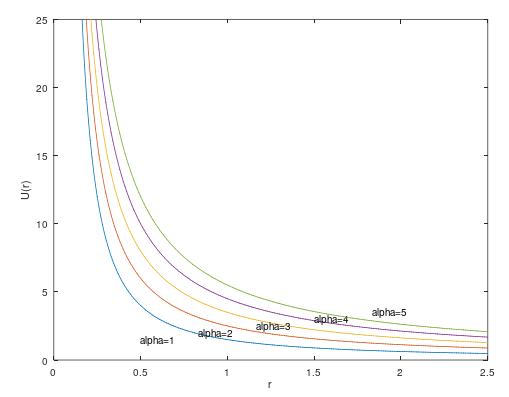
\includegraphics[width=10cm]{chapter_03_paragraph_15_fig_13a}
		\caption{\'Energie potentielle r\'epulsive pour $\alpha\in \{1;2;3;4;5\}$ et $M^{2}/m = 1$}\label{FIG:3_13a}
	\end{center}
\end{figure}

L'\'energie de la particule en jeu est de facto strictement positive \`a la vue de la courbe obtenue pour l'\'energie potentielle, sachant que l'\'energie cin\'etique est toujours positive. En reprenant l'\'equation (\ref{EQ:14_7}), soit :
\be
	\varphi = \bigintsss{\dfrac{\frac{M}{r^{2}}\mathrm{d}r}{\sqrt{2m\left(E + \dfrac{\alpha}{r}\right) - \frac{M^{2}}{r^{2}}}}}
\ee
et en substituant la quantit\'e $\alpha$ par $-\alpha$, nous obtenons :
\be
	\cos\varphi = \dfrac{\dfrac{M}{r} + \dfrac{m\alpha}{M}}{\sqrt{2mE + \dfrac{m^{2}\alpha^{2}}{M^{2}}}}
\ee
Avec les relations (\ref{EQ:15_4}), nous obtenons ici :
\bea
	\cos\varphi & = & \dfrac{\dfrac{p}{r} + 1}{e} \nonumber \\
	\dfrac{p}{r} & = & -1 + e\cos\varphi \label{EQ:15_14}
\eea
dont une repr\'esentation est sur la figure (\ref{FIG:3_13}). Nous pouvons aussi observer ici que $r$ est minimale quand la quantit\'e $\cos\varphi$ est maximale, donc le p\'erih\'elie s'\'ecrit ici :
\be
	r_{min} = \dfrac{p}{e - 1} = a(1 + e) \label{EQ:15_15}
\ee
car $a = \frac{\alpha}{2E}$.
L'\'equation (\ref{EQ:14_6}) se d\'eveloppe :
\be
	\mathrm{t} = \bigintsss{\dfrac{\mathrm{d}r}{\sqrt{\dfrac{2}{m}\left(E - \dfrac{\alpha}{r}\right) - \dfrac{M^{2}}{m^{2}r^{2}}}}} = \sqrt{\dfrac{ma}{\alpha}}\bigintsss{\dfrac{r\mathrm{d}r}{\sqrt{r^{2} - \dfrac{\alpha}{E}r - \dfrac{M^{2}}{2mE}}}}
\ee
En remarquant que :
\bea
	a^{2}e^{2} - (r - a)^{2} & = & a^{2}e^{2} - r^{2} - a^{2} + 2ar \nonumber \\
	& = & \dfrac{\alpha^{2}}{4E^{2}}\left(1 + \dfrac{2EM^{2}}{m\alpha^{2}}\right) - r^{2} - \dfrac{\alpha^{2}}{4E^{2}} + \dfrac{2\alpha r}{2E} \nonumber \\
	& = & -\left(r^{2} - \dfrac{\alpha}{E}r - \dfrac{M^{2}}{2mE}\right)
\eea
nous pouvons reprendre tel que :
\be
	\mathrm{t} = \sqrt{\dfrac{ma}{\alpha}}\bigintsss{\dfrac{r\mathrm{d}r}{\sqrt{(r - a)^{2} - a^{2}e^{e}}}}
\ee
En posant :
\be
	\begin{cases}
		r = a(e\cosh\xi + 1) \\
		\mathrm{d}r = ae\sinh\xi\mathrm{d}\xi
	\end{cases}
\ee
nous prolongeons en :
\bea
	\mathrm{t} & = & \sqrt{\dfrac{ma}{\alpha}}\bigintsss{\dfrac{a(e\cosh\xi + 1)ae\sin\xi\mathrm{d}\xi}{\sqrt{a^{2}e^{2}\cosh^{2}\xi - a^{2}e^{2}}}} = \sqrt{\dfrac{ma}{\alpha}}\bigintsss{\dfrac{a(e\cosh\xi + 1)ae\sin\xi\mathrm{d}\xi}{ae\sqrt{\cosh^{2}\xi - 1}}} \nonumber \\
	& = & \sqrt{\dfrac{ma^{3}}{\alpha}}\int{(e\cosh\xi + 1)\mathrm{d}\xi} \nonumber \\
	\mathrm{t} & = & \sqrt{\dfrac{ma^{3}}{\alpha}}(e\sinh\xi + \xi) \nonumber \\
\eea
Avec la m\^eme technique calculatoire que pr\'ec\'edemment, nous posons $x = r\cos\varphi$ et $y = r\sin\varphi$ et sachant (\ref{EQ:15_14}), nous avons :
\be
	p = a(e^{2} - 1)\text{ et }p + r = ex
\ee
donc :
\bea
	ex & = & a(e^{2} - 1) + a(e\cosh\xi + 1) = ae^{2} + ae\cosh\xi \nonumber \\
	\Leftrightarrow x & = & a(\cosh\xi + e)
\eea
et avec $y^{2} = r^{2} - x^{2}$ :
\bea
	y^{2} & = & a^{2}e^{2}\cosh^{2}\xi + a^{2} + 2ae\cosh\xi - a^{2}e^{2} - a^{2}\cosh^{2}\xi - 2ae\cosh\xi \nonumber \\
	& = & a^{2}e^{2}(1 + \sinh^{2}\xi) + a^{2} - a^{2}e^{2} - a^{2}(1 + \sinh^{2}\xi) \nonumber \\
	\Leftrightarrow y & = & a\sqrt{e^{2} - 1}\sinh\xi
\eea
avec $\xi \in ]-\infty ; +\infty[$. Nous avons ainsi la trajectoire param\'etrique telle que :
\be
	\begin{cases}
		r = a(e\cosh\xi + 1)\text{ et }\mathrm{t} = \sqrt{\dfrac{ma^{3}}{\alpha}}(e\sinh\xi + \xi) \\
		x = a(\cosh\xi + e)\text{ et }y = a\sqrt{e^{2} - 1}\sinh\xi \label{EQ:15_16}
	\end{cases}
\ee

\subsection{Int\'egrale sp\'ecifique du champ en $\alpha/r$}

Cherchons une int\'egrale premi\`ere, i.e. constante dans le temps, sp\'ecifique \`a ce type de champ en $\frac{\alpha}{r}$ avec $\alpha\in\mathbb{R}$ en remarquant que :
\bea
	\dfrac{\mathrm{d}}{\mathrm{dt}}\left(\vec{v}\wedge\vec{M} + \dfrac{\alpha}{r}\vec{r}\right) & = & \vec{\dot{v}}\wedge\vec{M} + \vec{v}\wedge\vec{\dot{M}} + \dfrac{\alpha}{r}\vec{\dot{r}} - \dfrac{\alpha}{r^{3}}\vec{r}(\vec{v}\cdot\vec{r}) \nonumber \\
	& = & \vec{\dot{v}}\wedge\vec{M} + \dfrac{\alpha}{r}\vec{\dot{r}} - \dfrac{\alpha}{r^{3}}\vec{r}(\vec{v}\cdot\vec{r})
\eea
car il y a toujours conservation du moment cin\'etique et donc $\vec{\dot{M}} = \vec{0}$. De plus $\vec{M} = m\vec{r}\wedge\vec{v}$ donc :
\be
	\dfrac{\mathrm{d}}{\mathrm{dt}}\left(\vec{v}\wedge\vec{M} + \dfrac{\alpha}{r}\vec{r}\right)  = m(\vec{\dot{v}}\cdot\vec{v})\vec{r} - m(\vec{\dot{v}}\cdot\vec{r})\vec{v} + \dfrac{\alpha}{r}\vec{\dot{r}} - \dfrac{\alpha}{r^{3}}\vec{r}(\vec{v}\cdot\vec{r})
\ee
En revenant à l'\'equation du mouvement (\ref{EQ:5_3}) :
\be
	m\vec{\dot{v}} = -\dfrac{\partial U}{\partial\vec{r}} = \dfrac{\alpha}{r^{3}}\vec{r}
\ee
La quantit\'e :
\bea
	m(\vec{\dot{v}}\cdot\vec{v})\vec{r} - m(\vec{\dot{v}}\cdot\vec{r})\vec{v} + \dfrac{\alpha}{r}\vec{\dot{r}} - \dfrac{\alpha}{r^{3}}\vec{r}(\vec{v}\cdot\vec{r}) & = & m(\vec{\dot{v}}\cdot\vec{v})\vec{r} - m(\vec{\dot{v}}\cdot\vec{r})\vec{v} + \dfrac{\alpha}{r}\vec{\dot{r}} - m\vec{\dot{v}}(\vec{v}\cdot\vec{r}) \nonumber \\
	& = & m(\vec{\dot{v}}\cdot\vec{v})\vec{r} - m\vec{\dot{v}}(\vec{v}\cdot\vec{r}) - (m\vec{\dot{v}}\cdot\vec{r})\vec{v} + \dfrac{\alpha}{r}\vec{\dot{r}} \nonumber \\
	& = & m(\vec{\dot{v}}\cdot\vec{v})\vec{r} - m(\vec{\dot{v}}\cdot\vec{v})\vec{r} - \dfrac{\alpha}{r}\vec{v} + \dfrac{\alpha}{r}\vec{\dot{r}} \nonumber \\
	& = & \vec{0}
\eea
Ainsi le vecteur :
\be
	\vec{v}\wedge\vec{M} + \dfrac{\alpha}{r}\vec{r} = \vec{cste} \label{EQ:15_17}
\ee
se conserve dans le temps, en direction et en norme. Par d\'efinition, le vecteur $\vec{v}\wedge\vec{M}$ a la m\^eme direction que $\vec{r}$ et \`a la position du p\'erih\'elie, la vitesse radiale est nulle, donc le vecteur conservatif d\'efinit par (\ref{EQ:15_17}) est dirig\'e vers le grand axe du foyer. De plus, au p\'erih\'elie, nous avons $r = r_{min}$ par d\'efinition et la composante radiale de la vitesse de la particule est nulle. Aussi, la quantité (\ref{EQ:15_17}) se d\'eveloppe au p\'erih\'elie ainsi :
\be
	\vec{v}\wedge\vec{M} + \dfrac{\alpha}{r}\vec{r} = \begin{pmatrix} 0 \\ v_{\varphi} \\ 0 \end{pmatrix} \wedge \begin{pmatrix} 0 \\ 0 \\ M_{z} \end{pmatrix} + \begin{pmatrix} \alpha \\ 0 \\ 0 \end{pmatrix} = \begin{pmatrix} v_{\varphi}M_{z} + \alpha \\ 0 \\ 0 \end{pmatrix}
\ee
avec $v_{\varphi}$ la vitesse selon $\varphi$ au p\'erih\'elie. Or l'\'equation (\ref{EQ:14_2}) donne $M = mr^{2}\dot{\varphi}$ ou encore dans notre cas \`a la position du p\'erih\'elie, $M_{z} = M = mr_{min}^{2}\dot{\varphi}$. Cette relation peut aussi s'\'ecrire :
\bea
	\dfrac{\mathrm{d}\varphi}{\mathrm{dt}} & = & \dfrac{M}{mr_{min}^{2}} \nonumber \\
	v_{\varphi} & = & \dfrac{M}{mr_{min}}
\eea
car $v_{\varphi} = r_{min}\dot{\varphi}$. La quantité :
\bea
	v_{\varphi}M_{z} + \alpha & = & \dfrac{M^{2}}{mr_{min}} + \alpha = \dfrac{M^{2}(e - 1)}{mp} + \alpha \nonumber \\
	& = & \dfrac{M^{2}(e - 1)m\alpha}{mM^{2}} + \alpha = (e - 1)\alpha + \alpha \nonumber \\
	& = & \alpha e
\eea
en prenant pour r\'ef\'erence pour la valeur du param\`etre $p$ la relation (\ref{EQ:15_15}). Le vecteur d\'efini en (\ref{EQ:15_17}) est donc constant en norme qui est \'egale \`a $\alpha e$. L'int\'egrale premi\`ere (\ref{EQ:15_17}) comme les lois de conservation de l'\'energie et du moment cin\'etique est une fonction uniforme de l'\'etat de la particule, position et vitesse. L'apparition de l'int\'egrale (\ref{EQ:15_17}) suppl\'ementaire est due à la d\'eg\'en\'erescence du mouvement, \'etudi\'e au paragraphe (\ref{PAR:50}).